\section*{Preparatory questions}
\thispagestyle{empty}

\subsection*{Question 1}

Generating a Mandelbrot set is not an equilibrated task. Indeed some
pixels need more computation than others. Pixels are generated via the method 
\textit{is\_in\_Mandelbrot} 
which consists in a loop bounded by a given number of iteration
\textit{maxiter} and a distance \textit{dist2}. If the distance is superior
than 4, the computation stops and the pixel is not part of the Mandelbrot
set. However if this pixel is actually part of the set the computation stops
when \textit{maxiter} is reached, which implies more computation. 
This results in an unbalanced workload. 

\subsection*{Question 2}

The naive load-balancing method consists in dividing the picture same size 
blocks, each assigned to a thread. For example, running the program with two
threads results in dividing the the workload in two equal parts. Obviously
this method is unbalanced.
A better solution would be to divide the work in way smaller parts, a 
square or a rectangle of (x,y) pixels resulting in a lot more \textit{workunit}
than the number of threads.
This way, each thread would compute a tiny piece of work, and after completion
look for another one among the remaining workload. A system of mutex has to
be implemented to protect the work assignation.
Statistically this method provides a more balanced computation because each of
them will process \textit{hard} and \textit{easy} parts.

\vspace*{1em}
\begin{figure}[h]
    \centering
 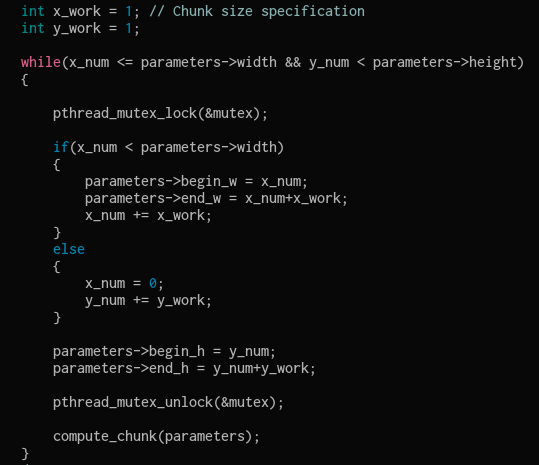
\includegraphics[width=.70\linewidth,scale=1]{./images/0.png} 
    \caption{Load-balanced implementation}
\end{figure}
\newpage
\thispagestyle{empty}

\section*{Performance results and comparison}
\subsection*{On our laptop(i5 2520M, 2Cores 4Threads)}

On the following figures, we cleary notice that the workload is unbalanced
with the \textit{naive} solution, for example the computation is actually
slower using 3 threads rather than 2.
On the other hand, with our balanced implementation the workload 
scale with the number of threads.

Note that with this 2C/4T machine we observe slower performances while 
using 5 or 6 threads, which is normal since the computation is using more 
threads that the machine actually has.

\begin{figure}[h]
    \centering
    \begin{tabular}{cc}
 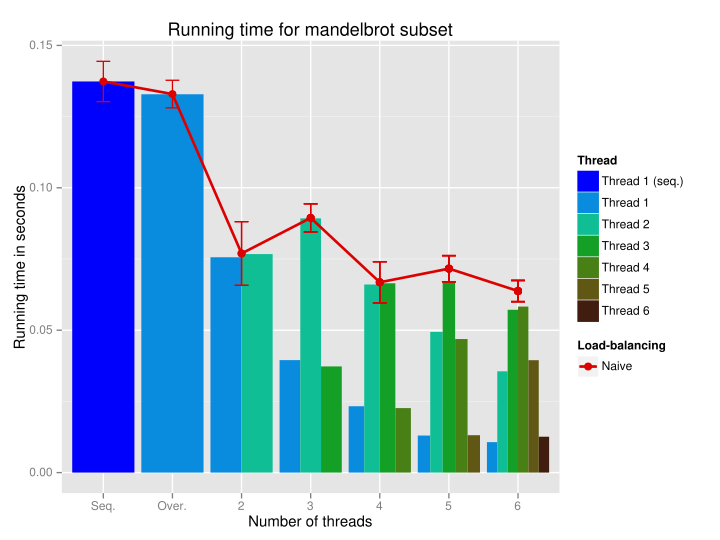
\includegraphics[width=.50\linewidth,scale=1]{./images/2.png} &
 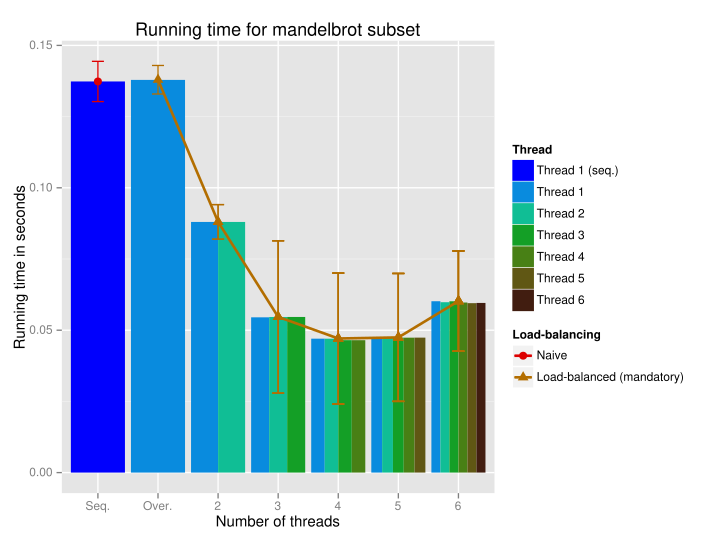
\includegraphics[width=.50\linewidth, scale=1.5]{./images/3.png} \\
      (a) & (b)
    \end{tabular}
    \caption{Naive (a) and Load-balanced (b)}
\end{figure}

\subsection*{On a multicore lab computer}


\begin{figure}[h]
    \centering
    \begin{tabular}{cc}
 %\includegraphics[width=.49\linewidth,scale=1]{./images/tab3.png} &
 %\includegraphics[width=.49\linewidth, scale=1.5]{./images/tab4.png} \\
      (a) & (b)
    \end{tabular}
    \caption{Naive (a) and Load-balanced (b)}
\end{figure}








